\documentclass[a4paper,cs4size]{BHCexam}
%\documentclass[a4paper,cs4size,answers]{BHCexam}

\usepackage{multicol} % 分栏
\usepackage{hyperref}
\pagestyle{fancy}
\fancyfoot[C]{\kaishu \small 第 \thepage 页 共 \pageref{lastpage} 页}
%\fancyhead[L]{\includegraphics[width=2cm]{qrcode.png}}
\title{电路习题课5}
%\subtitle{数学文科试卷}
%\notice{满分150分, 120分钟完成, \\	允许使用计算器,答案一律写在答题纸上.}
%\author{Gavin Chen}
%\date{\today}

\begin{document}
\maketitle
\begin{groups}

    \group{}{例题}
    %\zihao{-4}
    \begin{questions}[]

        \question[5] 要使电热器的发热功率减小一半,应该(\quad\quad\quad)。
        \fourchoices{使加给它两端的电压减小一半}
        {使它的电阻减小一半}
        {让通过它的电流减小一半}
        {使它的电阻和两端的电压同时减小一半}
        \vspace{2.5cm}



        \question[5] 在如图所示的电路中,电源电压保持不变。闭合开关$S$,当滑片$P$置于滑动变阻器的中点时,
        电压表的示数为$4V$;当滑片置于滑动变阻器的$b$端时,电压表的示数变化了$2V$,此后$15s$ 内定值电阻 $R_1$产生的热量为$60J$。
        下列结果中正确的是(\quad\quad\quad)。
        \fourchoices{电源电压为$10V$}
        {$R_1$的阻值为$18\Omega$}
        {滑动变阻器R的最大阻值为$9\Omega$}
        {$R_1$先后两次消耗的电功率之比为$4:3$}
        \begin{figure}[htb]
            \flushright
            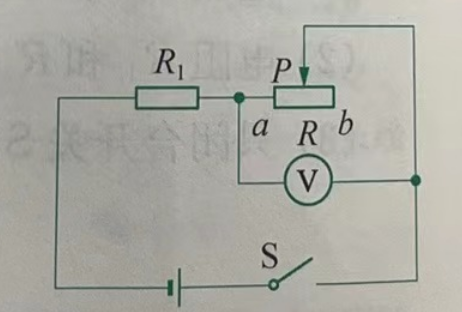
\includegraphics [scale=0.45,trim=0 0 0 0]{./image/physics_circuit5_1.png}
            % \caption{例1图}
            \label{fig:fig_circuit5_1}
        \end{figure}
        \vspace{2.5cm}

        \question[5] 明准备参加玩具赛车比赛,他利用如图所示的电路来挑选一只能量转换效率较高的电动机。
        设电池的电压恒定不变,他先用手捏住电动机的转轴,使其不转动,闭合开关后读出电流表的读数为$2A$;
        然后放手,当电动机正常转动时,又读出电流表的读数为$0.6A$。则该玩具电动机正常转动时的效率为是多少?
        \begin{figure}[htb]
            \flushright
            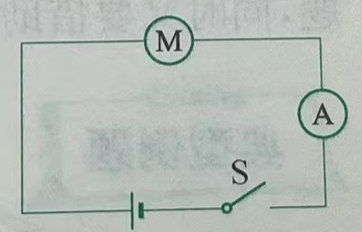
\includegraphics [scale=0.6,trim=0 0 0 0]{./image/physics_circuit5_2.png}
            % \caption{例1图}
            \label{fig:fig_circuit5_2}
        \end{figure}
        \vspace{2.5cm}

        \question[5] 用一个小型电动机提升重物,当给定电压为$2V$时,电机没有转动,此时通过电机的电流为$1A$。
        当电压增加到$12V$ 时,电机开始工作,此时电机能带动$16N$重的物体以$1m/s$的速度匀速上升。
        则下列判断中正确的是(\quad\quad\quad)。
        \fourchoices{电机的工作电流一定为$4A$}
        {电机线圈阻值为$12\Omega$}
        {电机的损耗功率可能为$8W$}
        {电机的效率可能为$50\%$}
        \vspace{2.5cm}


        \question[5] 如图所示,两根相互平行的长直导线分别通有方向相反的电流$I_1$和$I_2$,且$I_1>I_2$。
        $a$、$b$、$c$、$d$为导线某一横截面所在平面内的四点,且$a$、$b$、$c$与两导线共面,$b$、$d$的连线与导线所在
        平面垂直。磁感应强度可能为零的点是(\quad\quad\quad)。
        \fourchoices{$a$点}{$b$点}{$c$点}{$d$点}
        \begin{figure}[htb]
            \flushright
            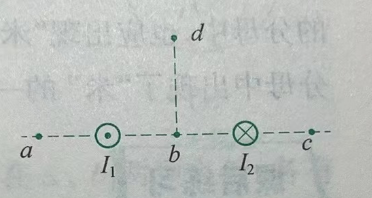
\includegraphics [scale=0.7,trim=0 0 0 0]{./image/physics_circuit5_3.png}
            % \caption{例1图}
            \label{fig:fig_circuit5_3}
        \end{figure}
        \vspace{2.5cm}

        \question[5] 如图所示,一束粒子沿水平方向飞过小磁针的下方,此时小磁针的$N$极向纸内偏转,这一束粒子可能是(\quad\quad\quad)。
        \fourchoices{向右飞行的正离子束}
        {向左飞行的负离子束}
        {向右飞行的电子束}
        {向左飞行的电子束}
        \begin{figure}[htb]
            \flushright
            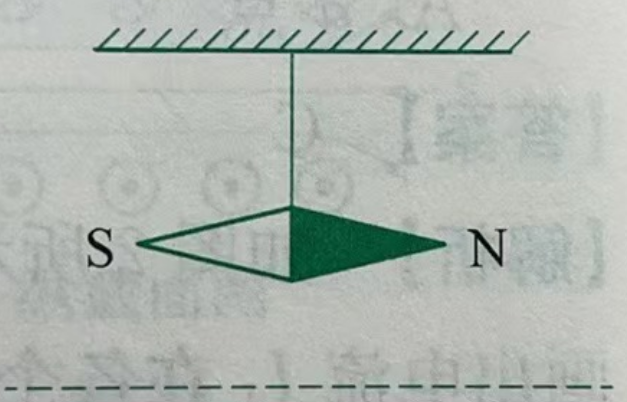
\includegraphics [scale=0.4,trim=0 0 0 0]{./image/physics_circuit5_4.png}
            % \caption{例1图}
            \label{fig:fig_circuit5_4}
        \end{figure}
        \vspace{2.5cm}

        \question[5] 奥斯特做电流磁效应实验时应排除地磁场对实验的影响,下列关于奥斯特实验的说法中正确的是(\quad\quad\quad)。
        \fourchoices{通电直导线必须竖直放置}
        {该实验必须在地球赤道上进行}
        {通电直导线应该水平东西方向放置}
        {通电直导线可以水平南北方向放置}
        \vspace{2.5cm}

        \question[5] 当导线中分别通以如图所示各方向的电流时,小磁针静止时$N$极指向读者的是(\quad\quad\quad)。
        \begin{figure}[htb]
            \center
            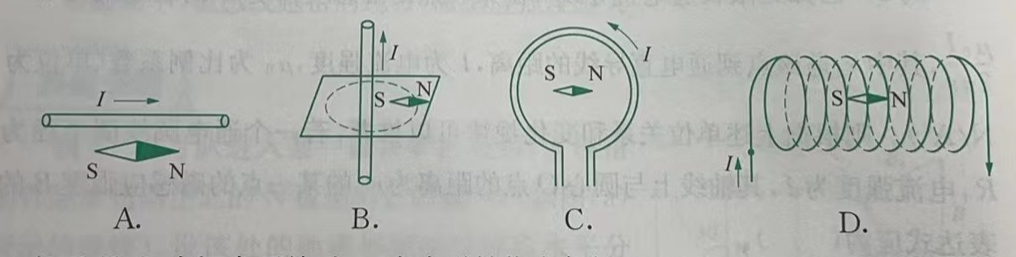
\includegraphics [scale=0.7,trim=0 0 0 0]{./image/physics_circuit5_5.png}
            % \caption{例1图}
            \label{fig:fig_circuit5_5}
        \end{figure}
        \vspace{2.5cm}

        \question[5]如图所示,当闭合开关后,四个小磁针指向都标正确的图是(\quad\quad\quad)。
        \begin{figure}[htb]
            \center
            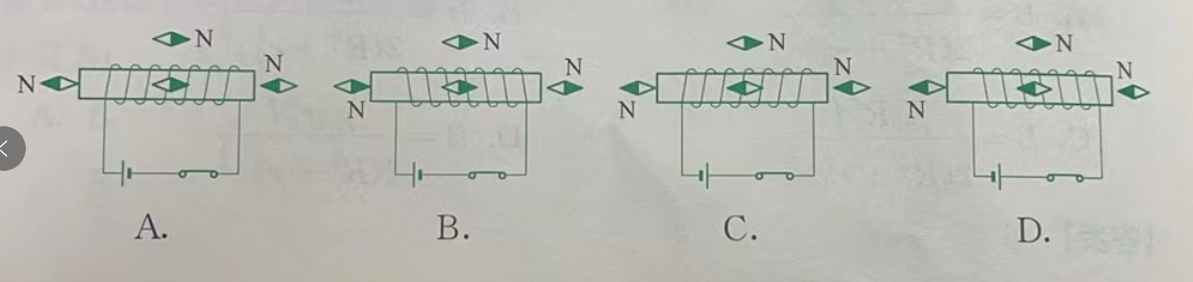
\includegraphics [scale=0.6,trim=0 0 0 0]{./image/physics_circuit5_8.png}
            % \caption{例1图}
            \label{fig:fig_circuit5_8}
        \end{figure}
        \vspace{2.5cm}


        \question[5] 为了解释地球的磁性,在$19$世纪,安培假设地球的磁场是由绕过地心的轴的环形电流引起的。
        下图中能正确表示安培假设中环形电流$I$方向的是(\quad\quad\quad)。
        \begin{figure}[htb]
            \center
            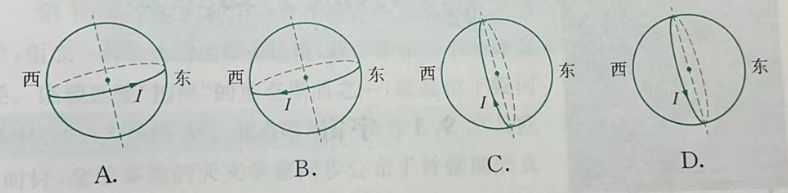
\includegraphics [scale=0.85,trim=0 0 0 0]{./image/physics_circuit5_6.png}
            % \caption{例1图}
            \label{fig:fig_circuit5_6}
        \end{figure}
        \vspace{2.5cm}

        \question[5] 如图所示,$a$、$b$、$c$为纸面内等边三角形的三个顶点,在$a$、$b$两顶点处,各有一条长直导线垂直穿过纸面,
        导线中通有大小相等的恒定电流,方向垂直于纸面向里,则$c$点的磁感应强度$B$的方向为(\quad\quad\quad)。
        \fourchoices{与$ab$边平行,向上}
        {与$ab$边平行,向下}
        {与$ab$边垂直,向右}
        {与$ab$边垂直,向左}
        \begin{figure}[htb]
            \flushright
            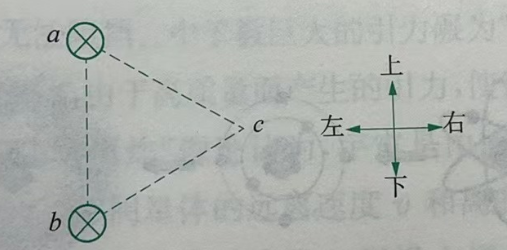
\includegraphics [scale=0.5,trim=0 0 0 0]{./image/physics_circuit5_7.png}
            % \caption{例1图}
            \label{fig:fig_circuit5_7}
        \end{figure}


    \end{questions}





\end{groups}


\label{lastpage}
\end{document}
